% Options for packages loaded elsewhere
\PassOptionsToPackage{unicode}{hyperref}
\PassOptionsToPackage{hyphens}{url}
\PassOptionsToPackage{dvipsnames,svgnames,x11names}{xcolor}
\documentclass[
  11pt,
]{article}
\usepackage{xcolor}
\usepackage[margin=1in]{geometry}
\usepackage{amsmath,amssymb}
\setcounter{secnumdepth}{5}
\usepackage{iftex}
\ifPDFTeX
  \usepackage[T1]{fontenc}
  \usepackage[utf8]{inputenc}
  \usepackage{textcomp} % provide euro and other symbols
\else % if luatex or xetex
  \usepackage{unicode-math} % this also loads fontspec
  \defaultfontfeatures{Scale=MatchLowercase}
  \defaultfontfeatures[\rmfamily]{Ligatures=TeX,Scale=1}
\fi
\usepackage{lmodern}
\ifPDFTeX\else
  % xetex/luatex font selection
\fi
% Use upquote if available, for straight quotes in verbatim environments
\IfFileExists{upquote.sty}{\usepackage{upquote}}{}
\IfFileExists{microtype.sty}{% use microtype if available
  \usepackage[]{microtype}
  \UseMicrotypeSet[protrusion]{basicmath} % disable protrusion for tt fonts
}{}
\makeatletter
\@ifundefined{KOMAClassName}{% if non-KOMA class
  \IfFileExists{parskip.sty}{%
    \usepackage{parskip}
  }{% else
    \setlength{\parindent}{0pt}
    \setlength{\parskip}{6pt plus 2pt minus 1pt}}
}{% if KOMA class
  \KOMAoptions{parskip=half}}
\makeatother
\usepackage{longtable,booktabs,array}
\newcounter{none} % for unnumbered tables
\usepackage{calc} % for calculating minipage widths
% Correct order of tables after \paragraph or \subparagraph
\usepackage{etoolbox}
\makeatletter
\patchcmd\longtable{\par}{\if@noskipsec\mbox{}\fi\par}{}{}
\makeatother
% Allow footnotes in longtable head/foot
\IfFileExists{footnotehyper.sty}{\usepackage{footnotehyper}}{\usepackage{footnote}}
\makesavenoteenv{longtable}
\usepackage{graphicx}
\makeatletter
\newsavebox\pandoc@box
\newcommand*\pandocbounded[1]{% scales image to fit in text height/width
  \sbox\pandoc@box{#1}%
  \Gscale@div\@tempa{\textheight}{\dimexpr\ht\pandoc@box+\dp\pandoc@box\relax}%
  \Gscale@div\@tempb{\linewidth}{\wd\pandoc@box}%
  \ifdim\@tempb\p@<\@tempa\p@\let\@tempa\@tempb\fi% select the smaller of both
  \ifdim\@tempa\p@<\p@\scalebox{\@tempa}{\usebox\pandoc@box}%
  \else\usebox{\pandoc@box}%
  \fi%
}
% Set default figure placement to htbp
\def\fps@figure{htbp}
\makeatother
% definitions for citeproc citations
\NewDocumentCommand\citeproctext{}{}
\NewDocumentCommand\citeproc{mm}{%
  \begingroup\def\citeproctext{#2}\cite{#1}\endgroup}
\makeatletter
 % allow citations to break across lines
 \let\@cite@ofmt\@firstofone
 % avoid brackets around text for \cite:
 \def\@biblabel#1{}
 \def\@cite#1#2{{#1\if@tempswa , #2\fi}}
\makeatother
\newlength{\cslhangindent}
\setlength{\cslhangindent}{1.5em}
\newlength{\csllabelwidth}
\setlength{\csllabelwidth}{3em}
\newenvironment{CSLReferences}[2] % #1 hanging-indent, #2 entry-spacing
 {\begin{list}{}{%
  \setlength{\itemindent}{0pt}
  \setlength{\leftmargin}{0pt}
  \setlength{\parsep}{0pt}
  % turn on hanging indent if param 1 is 1
  \ifodd #1
   \setlength{\leftmargin}{\cslhangindent}
   \setlength{\itemindent}{-1\cslhangindent}
  \fi
  % set entry spacing
  \setlength{\itemsep}{#2\baselineskip}}}
 {\end{list}}
\usepackage{calc}
\newcommand{\CSLBlock}[1]{\hfill\break\parbox[t]{\linewidth}{\strut\ignorespaces#1\strut}}
\newcommand{\CSLLeftMargin}[1]{\parbox[t]{\csllabelwidth}{\strut#1\strut}}
\newcommand{\CSLRightInline}[1]{\parbox[t]{\linewidth - \csllabelwidth}{\strut#1\strut}}
\newcommand{\CSLIndent}[1]{\hspace{\cslhangindent}#1}
\setlength{\emergencystretch}{3em} % prevent overfull lines
\providecommand{\tightlist}{%
  \setlength{\itemsep}{0pt}\setlength{\parskip}{0pt}}
\usepackage{setspace}
\setstretch{1.5}
\usepackage{indentfirst}
\setlength{\parindent}{10pt}
\usepackage{authblk}
\usepackage{booktabs}
\usepackage{caption}
\usepackage{dcolumn}
\usepackage{adjustbox}
\usepackage{threeparttable}
\usepackage{float}
\usepackage{fancyhdr}
\pagestyle{fancy}
\fancyhf{}
\setlength{\headheight}{14pt}
\fancyhead[L]{\small\scshape Online Appendix: Asymmetric Climate Impacts on Fishing Effort}
\fancyhead[R]{\small\thepage}
\renewcommand{\headrulewidth}{0.4pt}
\usepackage{etoolbox}
\author{Felipe J. Quezada-Escalona\thanks{Associate Professor, Department of Economics, Universidad de Concepci\'on. Mailing address: Victoria 471, Concepci\'on, Chile. Email: felipequezada@udec.cl. Adjunct Researcher, Interdisciplinary Center for Aquaculture Research---Applied Research (INCAR\textsuperscript{2}), Universidad de Concepci\'on.}}
\affil{Universidad de Concepci\'on \vspace{-60pt}}
\renewcommand{\thesection}{\Alph{section}}
\renewcommand{\thesubsection}{\Alph{section}.\arabic{subsection}}
\usepackage{chngcntr}
\counterwithin{table}{section}
\counterwithin{figure}{section}
\usepackage{bookmark}
\IfFileExists{xurl.sty}{\usepackage{xurl}}{} % add URL line breaks if available
\urlstyle{same}
\hypersetup{
  pdftitle={Differential Climate Impacts on Fishing Effort in Chilean Small Pelagic Fisheries},
  pdfauthor={Felipe J. Quezada-Escalona},
  colorlinks=true,
  linkcolor={blue},
  filecolor={Maroon},
  citecolor={blue},
  urlcolor={blue},
  pdfcreator={LaTeX via pandoc}}

\title{Differential Climate Impacts on Fishing Effort in Chilean Small Pelagic Fisheries}
\usepackage{etoolbox}
\makeatletter
\providecommand{\subtitle}[1]{% add subtitle to \maketitle
  \apptocmd{\@title}{\par {\large #1 \par}}{}{}
}
\makeatother
\subtitle{\begin{center}{\Large\textbf{Online Appendix}}\end{center}}
\author{Felipe J. Quezada-Escalona}
\date{June 2026}

\begin{document}
\maketitle

\doublespacing

\section{Reduced-form stress tests and prior elicitation}\label{appendix-stress}

This appendix describes how we set the priors on the climate shifters
\((\rho_s^{SST}, \rho_s^{CHL})\) that enter the state-space model of the
Stock dynamics subsection of the main text, together with the
identifiability diagnostic that motivates the use of Bayesian methods
over direct maximum likelihood.

\subsection{Deterministic hindcast and cross-variant fit}\label{sec:appendix-stress-spec}

For each stock \(s\) we estimate a deterministic Schaefer hindcast over
\(2000\)--\(2024\), \(\hat B_{s,t+1} = \hat B_{s,t} + r_{s,t}\hat B_{s,t}(1 - \hat B_{s,t}/K_s) - C_{s,t}\)
with \(r_{s,t} = r_s^{0} \exp(\rho_s^{SST}(SST_{t-1}-\overline{SST}) + \rho_s^{CHL}(\log CHL_{t-1}-\overline{\log CHL}))\),
stock-dynamics parameters \((r_s^{0}, K_s, B_{0,s})\) centred at the
IFOP/SPRFMO single-species priors, and shifters estimated by bounded
least squares on \([-3,3]^2\) minimising median absolute percent error
(MAPE). Four nested variants are reported: base (\(\rho=0\)), \(+\)SST
only, \(+\log\)CHL only, and joint \(+\)SST\(+\log\)CHL.
\label{eq:stress-law}
\label{eq:stress-shifter}
\label{sec:appendix-stress-results}

\begin{table}[!h]
\centering
\caption{\label{tab:stress-mape-table}Median absolute percent error of the deterministic Schaefer hindcast across shifter variants. \label{tab:stress-mape}}
\centering
\fontsize{10}{12}\selectfont
\begin{tabular}[t]{lrrrr}
\toprule
Stock & Base & + SST & + log CHL & + SST and log CHL\\
\midrule
Anchoveta & 95.9 & 30.8 & 95.1 & 26.6\\
Sardina com\'un & 98.5 & 23.1 & 98.5 & 20.5\\
Jack mackerel & 44.2 & 44.3 & 49.1 & 48.5\\
\bottomrule
\end{tabular}
\end{table}

No variant brings any of the three stocks below a \(20\%\) MAPE
threshold. The two coastal stocks benefit from activating SST
(anchoveta: \(95.9\%\to 30.8\%\), sardine: \(98.5\%\to 23.1\%\)), with
the joint specification delivering further marginal improvement.
Jack mackerel hindcast errors remain in the \(44\)--\(49\%\) range across
all variants, with no shifter distinguishably better than the base.

The joint-variant point estimates are internally coherent for the
coastal stocks. Anchoveta: both shifters negative and similar in
magnitude (\(\rho^{SST} \approx -2.3\), \(\rho^{CHL} \approx -2.3\)).
Sardina com\textquotesingle un: \(\rho^{SST} \approx -2.0\) but \(\rho^{CHL} \approx +2.1\)
(opposite sign for sardine, consistent with the established ecological
differentiation between sardine and anchoveta in the Humboldt system).
Jack mackerel: \(\rho^{SST} \approx +0.6\) small and the \(\rho^{CHL}\)
estimate binds at the lower boundary of the admissible box; we read
the boundary solution as a failure of point identification rather
than a finding of strong climate forcing.

\subsection{Identifiability diagnostic and prior elicitation}\label{sec:appendix-stress-diag}

\label{sec:appendix-stress-priors}

Two diagnostics motivate the use of weakly informative priors rather
than direct maximum-likelihood estimation. First, the two environmental
forcings are statistically orthogonal over the \(2000\)--\(2024\) sample
(Pearson \(r = 0.030\), \(p = 0.888\)), so the cross-variant gap in
hindcast error cannot be attributed to collinearity in the design
matrix. Second, the jurel MLE binds at the boundary: the deterministic
hindcast cannot separate the climate signal from process and observation
noise, so \(\rho\) is not separately identifiable. The Bayesian
state-space specification addresses both limitations within a single
estimation step.

Table \ref{tab:stress-priors} reports the priors on
\((\rho_s^{SST}, \rho_s^{CHL})\) used in the structural likelihood.
Prior centres for the two coastal stocks are the joint MLEs rounded to
one decimal place; jurel priors are centred at zero so that posterior
identification is driven by the structural likelihood rather than by
the boundary solution. All priors are independent normal with unit
standard deviation; no hierarchical pooling is imposed because
\(\rho^{CHL}\) switches sign between anchoveta and sardine.

This prior-elicitation strategy is a form of empirical Bayes: the
prior centres for anchoveta and sardine are derived from the same
2000--2024 biomass series that enters the state-space likelihood,
which trades pure data-prior independence for tractable identification
under \(N=25\) annual observations. We adopt this trade-off deliberately
for two reasons. First, the prior standard deviation \(\sigma = 1\) is
large enough that the posterior is free to move substantially: the
posterior of \(\rho_s^{CHL}\) for anchoveta migrates to \(-3.65\)
(prior mean \(-2.3\)), more than one prior standard deviation from
the centre, illustrating that the data does refine the prior when
informative. Second, the alternative of centring all priors at zero
would, under \(N=25\), leave the joint posterior of
\((r_s^{0}, K_s, B_{0,s}, \rho_s^{SST}, \rho_s^{CHL})\) weakly identified
or multimodal, producing posteriors that are uninformative for
projections regardless of whether the underlying coupling is real or
absent. The empirical-Bayes choice therefore makes the non-identification
result for jack mackerel a substantive finding rather than a numerical
artefact of weak posterior geometry.

\begin{table}[!h]
\centering
\caption{\label{tab:stress-priors-table}Independent normal priors on the climate shifters used in the state-space likelihood. \label{tab:stress-priors}}
\centering
\fontsize{10}{12}\selectfont
\begin{tabular}[t]{lrrrrl}
\toprule
Stock & $\mu_{\rho^{SST}}$ & $\sigma_{\rho^{SST}}$ & $\mu_{\rho^{CHL}}$ & $\sigma_{\rho^{CHL}}$ & Source\\
\midrule
Anchoveta & -2.3 & 1.0 & -2.3 & 1.0 & Joint MLE\\
Sardina com\'un & -2.0 & 1.0 & +2.1 & 1.0 & Joint MLE\\
Jack mackerel & 0.0 & 1.0 & 0.0 & 1.0 & Boundary solution; vague prior\\
\bottomrule
\end{tabular}
\end{table}

\section{Predictive diagnostics}\label{appendix-predictive}

This appendix reports the nested predictive comparison referenced in
the Stock dynamics subsection of the main text, comparing three state-space
specifications: (i) species-independent dynamics without climate
shifters (\emph{ind}), (ii) the same with a cross-stock residual
covariance \(\Omega\) (\emph{omega}), and (iii) the full model
augmented with the climate shifter of Eq.\textasciitilde(1) of the main text
(\emph{full}). Two predictive metrics are reported: leave-one-out
PSIS-LOO (Pareto-smoothed importance sampling) and one-step-ahead LFO
(leave-future-out).

\begin{table}[!h]
\centering
\caption{\label{tab:loo-appendix-table}PSIS-LOO comparison across state-space specifications. \label{tab:loo-appendix}}
\centering
\fontsize{10}{12}\selectfont
\begin{threeparttable}
\begin{tabular}[t]{lrrrrr}
\toprule
Model & $\widehat{\text{ELPD}}_{\text{loo}}$ & SE & $\Delta\widehat{\text{ELPD}}$ & SE$_{\Delta}$ & $\hat{p}_{\text{loo}}$\\
\midrule
T4b-full & -8.41 & 8.28 & -- & -- & 64.8\\
T4b-ind & -23.00 & 8.01 & -14.59 & 4.93 & 62.4\\
T4b-omega & -26.43 & 9.16 & -18.02 & 5.59 & 57.9\\
\bottomrule
\end{tabular}
\begin{tablenotes}
\item \textit{Note:} 
\item Δ ELPD is the pairwise difference relative to T4b-full (the leading model); the adjacent SE column reports the standard error of that difference. After moment matching, 65/68 observations satisfy Pareto-k <= 0.7 for T4b-full, 64/68 for T4b-ind, and 67/68 for T4b-omega. The remaining high-Pareto-k points are the two censored jack-mackerel years (2012, 2015), which appear in all three models and therefore do not affect the ranking.
\end{tablenotes}
\end{threeparttable}
\end{table}

PSIS-LOO favours the climate-augmented specification with a positive
\(\Delta\)ELPD of \(14\)--\(18\) relative to the climate-free specifications,
indicating that the in-sample predictive performance improves when the
climate shifter is included.

\begin{table}[!h]
\centering
\caption{\label{tab:lfo-appendix-table}One-step-ahead LFO comparison across state-space specifications. \label{tab:lfo-appendix}}
\centering
\fontsize{10}{12}\selectfont
\begin{threeparttable}
\begin{tabular}[t]{lcccrr}
\toprule
Model & Points & Censored & $\widehat{\text{ELPD}}_{\text{LFO}}$ & Mean per point & $\Delta$ vs leader\\
\midrule
T4b-full & 14 & 2 & -29.10 & -2.08 & --\\
T4b-ind & 14 & 2 & -29.46 & -2.10 & -0.37\\
T4b-omega & 14 & 2 & -30.46 & -2.18 & -1.36\\
\bottomrule
\end{tabular}
\begin{tablenotes}
\item \textit{Note:} 
\item Sum of one-step predictive log densities over five origin years (2011, 2014, 2017, 2020, 2022) and three stocks (14 targets per model; two are censored). Each refit uses 4 chains × 1500 warmup + 1500 sampling iterations. All 15 refits satisfied R-hat <= 1.01 with at most one divergent transition (T4b-omega at the 2011 origin), which does not affect the reported ELPD.
\end{tablenotes}
\end{threeparttable}
\end{table}

The one-step-ahead LFO comparison is essentially a tie across the three
specifications, indicating that the climate-augmented specification does
not deliver a detectable improvement in short-horizon forecast
performance over the climate-free alternatives. We interpret this as a
sample-size issue rather than a deficiency of the climate
specification: the structural climate elasticities are identified on
the full \(25\)-year window, not on one-step-ahead increments. The
posterior of the climate-augmented specification remains our primary
object of interpretation in the main text.

\section{Posterior-predictive checks}\label{appendix-posterior}

This appendix reports posterior-predictive diagnostics of the full
state-space specification: (i) the smoothed latent biomass versus the
observed survey-based estimates, and (ii) the corresponding year-level
residuals.

\begin{figure}[H]
\centering
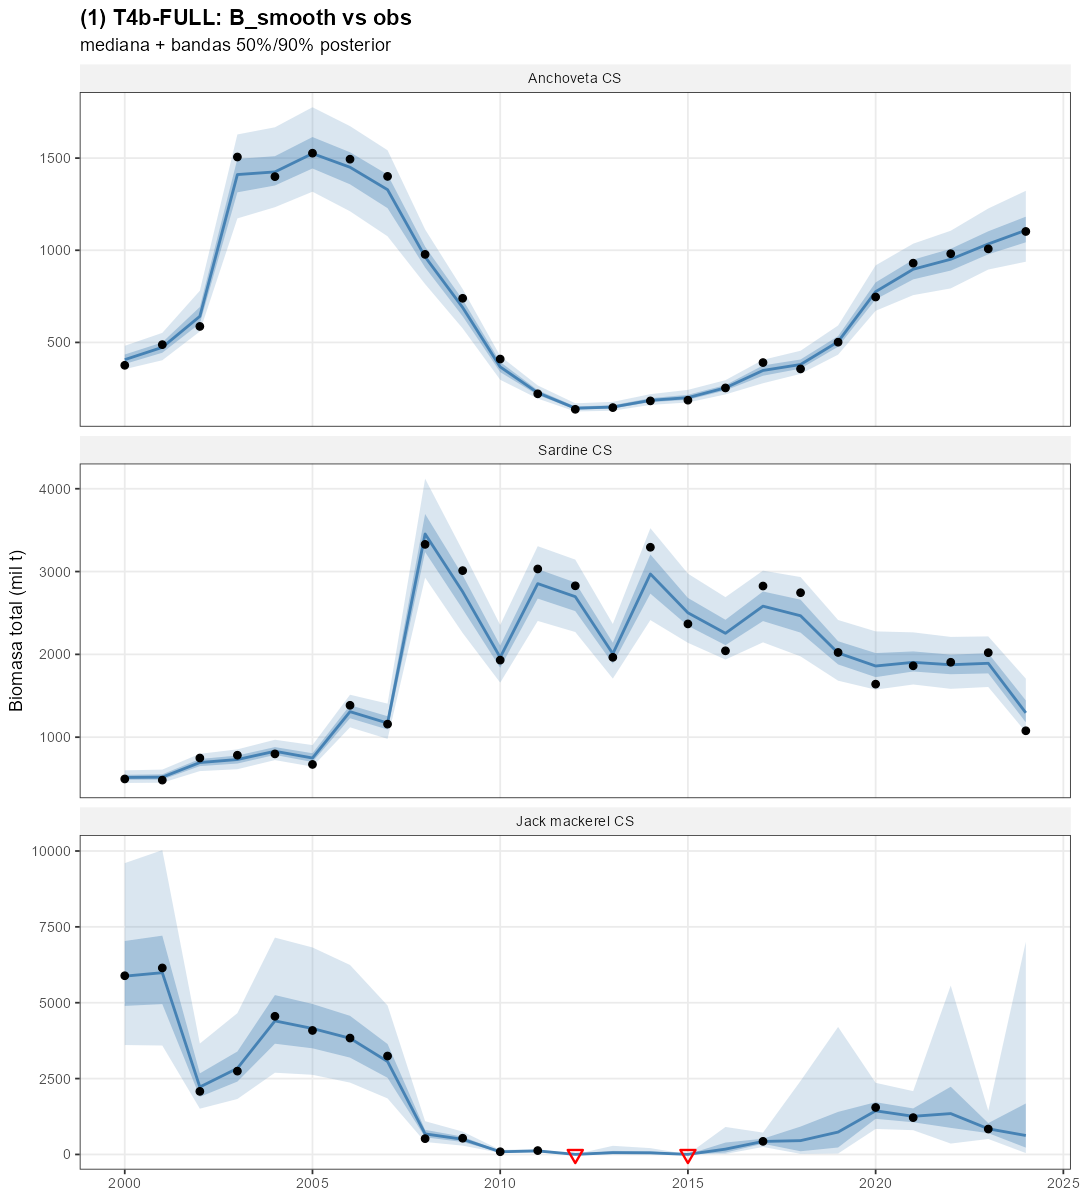
\includegraphics[width=0.95\textwidth]{../figs/t4b/t4b_full_smooth_vs_obs.png}
\caption{Smoothed latent biomass $B_{i,t}$ of the full specification
against survey-based SSB observations, by stock. Solid line: posterior
median; shaded band: $90\%$ credible interval. Open circles: official
IFOP/SPRFMO point estimates; downward arrows: left-censored
observations at the assessment detection limit (jurel $2012$,
$2015$).\label{fig:ppc-smooth-vs-obs}}
\end{figure}

The smoothed band has a median width of approximately \(20\%\) of the
posterior mean, tightening over years with direct observation and
widening across the seven non-surveyed jurel years (latent biomass
identified dynamically through the Schaefer transition and two censored
observations in \(2012\) and \(2015\)).

\begin{figure}[H]
\centering
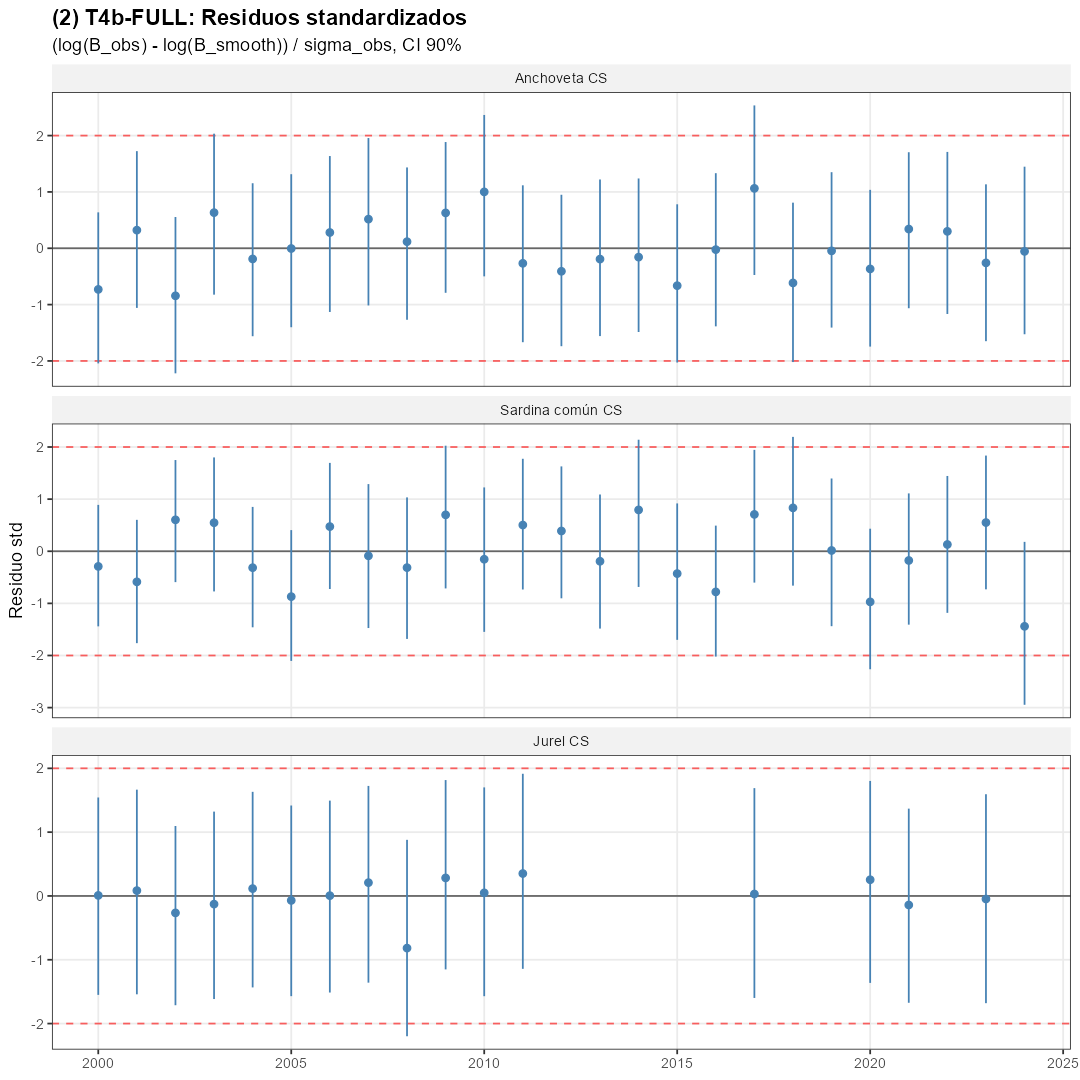
\includegraphics[width=0.95\textwidth]{../figs/t4b/t4b_full_residuals.png}
\caption{Standardised year-level residuals of the full specification by
stock. The Ljung--Box test of residual autocorrelation does not reject
the null at conventional levels for any of the three stocks.\label{fig:ppc-residuals}}
\end{figure}

\section{Markov-chain convergence diagnostics}\label{appendix-convergence}

Table \ref{tab:convergence} reports the Gelman--Rubin \(\hat{R}\) and
the bulk/tail effective sample sizes for the top-level parameters of
the full state-space specification, evaluated on four independent
Hamiltonian Monte Carlo chains of \(2{,}000\) post-warmup iterations
each. All \(\hat{R}\) values are below \(1.01\) and all effective sample
sizes exceed \(400\), indicating that posterior summaries are not
contaminated by between-chain divergence or by autocorrelation between
adjacent draws.

\begin{table}[!h]
\centering
\caption{\label{tab:convergence-table}Markov-chain convergence diagnostics for the top-level parameters of the T4b-full state-space specification. \label{tab:convergence}}
\centering
\fontsize{10}{12}\selectfont
\begin{threeparttable}
\begin{tabular}[t]{lrrrr}
\toprule
Parameter & $N$ & Max $\widehat{R}$ & Min ESS$_{\text{bulk}}$ & Min ESS$_{\text{tail}}$\\
\midrule
$r_i^{0}$ & 3 & 1.001 & 8,446 & 10,508\\
$K_i$ & 3 & 1.000 & 9,789 & 9,777\\
$B_{i,0}$ & 3 & 1.001 & 18,919 & 11,844\\
$\sigma_{\text{proc},i}$ & 3 & 1.003 & 3,353 & 5,997\\
$\sigma_{\text{obs},i}$ & 3 & 1.009 & 1,370 & 936\\
\addlinespace
$\rho_i^{SST}$ & 3 & 1.000 & 8,312 & 10,147\\
$\rho_i^{CHL}$ & 3 & 1.001 & 14,319 & 10,633\\
$\Omega$ (off-diagonal) & 3 & 1.001 & 5,732 & 8,544\\
\textit{All top-level parameters} & 24 & 1.009 & 1,370 & 936\\
\bottomrule
\end{tabular}
\begin{tablenotes}
\item \textit{Note:} 
\item Diagnostics are computed from four chains of 2,000 post-warmup iterations. Within each parameter family, the table reports the worst case across the three stocks (or the three off-diagonal entries of Omega): the largest split-Rhat and the smallest bulk- and tail-effective sample sizes. The diagonal of Omega is fixed at one and is therefore excluded. The conventional thresholds are Rhat <= 1.01 and ESS >= 400 for all top-level parameters.
\end{tablenotes}
\end{threeparttable}
\end{table}

\section{Spatial robustness of the jack mackerel non-identification result}\label{appendix-spatial}

The non-identification of \((\rho_{\text{jurel}}^{SST}, \rho_{\text{jurel}}^{CHL})\)
reported in the Identification of climate shifters section of the main text admits two observationally
equivalent readings: that jurel productivity is uncoupled from
Centro-Sur coastal forcing at the annual aggregate, or that the
relevant forcing operates at a spatial scale broader than the EEZ,
diluting the local-domain signal. This appendix tests four
explanations for the null --- insufficient power, insufficient
spatial extent, insufficient biomass coverage, and a poor choice of
spatial scale --- and concludes that the null is structural rather
than aggregation-driven within the \(2000\)--\(2024\) Centro-Sur record.

\subsection{Identification power on the sample}\label{sec:appendix-spatial-power}

Linearising the Schaefer transition in log-differences,
\(\Delta \log B_{i,t+1} = \alpha_i - \beta_i (B_{i,t}/K_i) + \rho_i^X X_{t-1} + \varepsilon_{i,t}\)
with \(\varepsilon_{i,t} \sim \mathcal{N}(0, \sigma_{i,\text{resid}}^2)\)
and \(\sigma_{i,\text{resid}} = \sqrt{\sigma_{i,\text{proc}}^2 + 2\sigma_{i,\text{obs}}^2}\),
the OLS-equivalent standard error on a sample of \(N=24\) lag-one
observations is
\(\mathrm{SE}(\hat{\rho}_i^X) \approx \sigma_{i,\text{resid}} / [\mathrm{sd}(X)\sqrt{N-K}]\)
with \(K=3\) regressors. The minimum shifter magnitude detectable at
\(80\%\) power for a two-sided \(90\%\) credible interval is then
\(|\rho_i^X|_{\min} \approx 2.56\,\mathrm{SE}(\hat{\rho}_i^X)\).

Evaluated at the posterior medians of \(\sigma_{\text{proc}}\) and
\(\sigma_{\text{obs}}\), \(\sigma_{i,\text{resid}}\) is \(0.28\) for
anchoveta, \(0.25\) for sardine, and \(1.28\) for jurel --- the latter
roughly \(4.6\) times the coastal-stock average and the main reason
why the prior dominates the jurel posterior. Table \ref{tab:appE-power}
reports \(|\rho|_{\min}\) for the three stocks and three candidate
shifters. The jurel envelope spans \(|\rho|_{\min}\) of \(1.50\) on
local SST, \(1.32\) on local \(\log\)\textasciitilde CHL, and \(0.71\) on basin-scale
ENSO, against an envelope of empirically plausible biological
elasticities centred near \(0.05\)--\(0.30\) in absolute value, far below the
\(|\rho|_{\min}\) envelope reported here. The sample is therefore insufficiently informative
to support a credible interval for jurel under any of these
forcings, regardless of the true elasticity.

\begin{table}[H]
\centering
\caption{Minimum shifter magnitude $|\rho|_{\min}$ detectable at
$80\%$ power on the $2000$--$2024$ sample.
$\sigma_{\text{resid}} = \sqrt{\sigma_{\text{proc}}^2 + 2\sigma_{\text{obs}}^2}$
evaluated at posterior medians.\label{tab:appE-power}}
\begin{threeparttable}
\begin{tabular}{lcccc}
\toprule
Stock & $\sigma_{\text{resid}}$ & $|\rho_{SST}|_{\min}$ & $|\rho_{\log\text{CHL}}|_{\min}$ & $|\rho_{\text{ENSO}}|_{\min}$ \\
\midrule
Anchoveta & $0.28$ & $0.33$ & $0.29$ & $0.16$ \\
Sardina común & $0.25$ & $0.29$ & $0.26$ & $0.14$ \\
Jurel & $1.28$ & $1.50$ & $1.32$ & $0.71$ \\
\bottomrule
\end{tabular}
\begin{tablenotes}[flushleft]\footnotesize
\item \emph{Notes.} Detectable magnitudes computed from
$|\rho_i^X|_{\min} \approx 2.56\,\sigma_{i,\text{resid}} / [\mathrm{sd}(X)\sqrt{N-K}]$
with $N=24$, $K=3$. $\mathrm{sd}(X)$ are sample standard deviations of
the Centro-Sur EEZ-aggregated SST and $\log$~CHL anomalies and of the
Niño 3.4 index over the estimation window.
\end{tablenotes}
\end{threeparttable}
\end{table}

\subsection{Posterior identification across alternative specifications}\label{sec:appendix-spatial-results}

We re-fit the state-space jurel block under four alternative shifter
configurations, each designed to test one mechanical explanation for
the local null. Table \ref{tab:appE-sigma} reports the
posterior-to-prior standard deviation ratios for the jurel shifters
under each specification; ratios at unity indicate no posterior
updating relative to the prior.

\begin{table}[H]
\centering
\caption{Posterior-to-prior standard deviation ratios of the jurel
climate shifters under four alternative specifications.\label{tab:appE-sigma}}
\begin{threeparttable}
\begin{tabular}{llcc}
\toprule
Test & Specification & $\sigma_{\text{post}}/\sigma_{\text{prior}}$ (SST) & $\sigma_{\text{post}}/\sigma_{\text{prior}}$ ($\log$~CHL or ENSO) \\
\midrule
Spatial extent & EEZ domain $\mathcal{D}_1$ & $0.998$ & $1.014$ ($\log$~CHL) \\
 & Offshore-extended $\mathcal{D}_2$ & $1.002$ & $1.009$ ($\log$~CHL) \\
 & Southeast Pacific $\mathcal{D}_3$ & $0.999$ & $1.011$ ($\log$~CHL) \\
Biomass coverage & Dual-source (Centro-Sur + Northern acoustic) & $0.94$ & $0.99$ ($\log$~CHL) \\
Spatial scale & Basin-scale ENSO Niño 3.4, lag~1 & --- & $0.98$ (ENSO) \\
 & Basin-scale ENSO Niño 3.4, lag~2 & --- & $1.01$ (ENSO) \\
Joint specification & Local SST + local $\log$~CHL + ENSO (lag~1) & $1.03$ & $1.00$ ($\log$~CHL); $0.98$ (ENSO) \\
\bottomrule
\end{tabular}
\begin{tablenotes}[flushleft]\footnotesize
\item \emph{Notes.} $\mathcal{D}_1$ is the Chilean EEZ between $18^{\circ}$S
and $42^{\circ}$S out to $200$ nautical miles. $\mathcal{D}_2$ extends to
$1{,}000$ km offshore. $\mathcal{D}_3$ is the regional Southeast Pacific
domain $5^{\circ}$S--$45^{\circ}$S, $70^{\circ}$W--$120^{\circ}$W.
Spatial aggregates are area-weighted (with $\cos(\text{lat})$) and
centred on the $2000$--$2024$ mean. The dual-source extension augments
the Centro-Sur biomass likelihood with the Northern Chilean acoustic
series under a common shifter $\rho_{\text{jurel}}^{\text{common}}$,
motivated by the $0.88$ log-scale cross-series correlation. The ENSO
specification replaces the local coastal shifters with the Niño 3.4
index at the indicated lag. The joint specification estimates all
three shifters simultaneously for jurel, holding the anchoveta and
sardina blocks at the main specification of the Stock dynamics subsection of the main text. Anchoveta and sardina shifter ratios remain
stable at $0.43$--$0.83$ across all configurations (not reported).
\end{tablenotes}
\end{threeparttable}
\end{table}

All four tests deliver a posterior-to-prior ratio between \(0.94\) and
\(1.03\) for the jurel shifters, statistically indistinguishable from
unity given the prior dispersion. The two ratios closest to ``informative
updating'' --- the dual-source extension at \(0.94\)--\(0.99\) and the
basin-scale ENSO at \(0.98\) --- remain well above the \(0.7\) threshold
below which posterior intervals discriminate the shifter from zero
on the prior support, consistent with the analytic power calculation
of Table \ref{tab:appE-power}.

\subsection{Dual-source extension}\label{sec:appendix-spatial-dual}

The Centro-Sur and Northern Chilean acoustic biomass series exhibit a
\(0.88\) log-scale correlation across overlapping years
(\(2012\)--\(2024\)), motivating a joint-likelihood specification in
which a common shifter \(\rho^{\text{common}}\) is identified
simultaneously on both records. The extension multiplies the number
of informative jurel-biomass observations by approximately \(1.7\)
while preserving the prior structure of the main fit. The resulting
\(\sigma_{\text{post}}/\sigma_{\text{prior}}\) ratios of \(0.94\)
(SST) and \(0.99\) (\(\log\)\textasciitilde CHL) are the strongest posterior updating
observed in any specification considered in this appendix, but
remain well above the threshold for material identification.

\subsection{Basin-scale ENSO test}\label{sec:appendix-spatial-enso}

Replacing the local coastal shifters with the basin-scale ENSO
Niño 3.4 index tests whether the relevant climatic forcing for
jurel operates at the basin scale rather than the coastal scale,
consistent with the empirical evidence of Peña-Torres et al. (\citeproc{ref-Pena-Torres2017-gn}{2017})
(ENSO-driven shifts in jurel location choices) and Arcos et al. (\citeproc{ref-Arcos2001-jq}{2001})
(SPRFMO-scale stock dynamics under broad-basin forcing). The
specification estimates a single \(\rho_{\text{jurel}}^{\text{ENSO}}\)
on lag-1 and lag-2 ENSO anomalies in alternative runs. The
resulting ratios of \(0.98\) (lag\textasciitilde1) and \(1.01\) (lag\textasciitilde2) are both
indistinguishable from unity, consistent with the analytic
\(|\rho_{\text{ENSO}}|_{\min} = 0.71\) of Table \ref{tab:appE-power}.

A prior-propagation sensitivity combines the posterior of
\(\rho_{\text{jurel}}^{\text{ENSO}}\) with the CMIP6 ensemble of
basin-scale temperature deltas to compute a \(90\%\) predictive
interval for the jurel productivity factor under SSP\(5\)-\(8.5\)
end-of-century. The interval spans approximately three orders of
magnitude (\([0.05, 19.5]\)), confirming that prior-propagated
projections are uninformative for policy and validating the
fixed-\(r^{\star}_{\text{jurel}}\) convention adopted in the main
text.

A separate exploratory attempt to incorporate the SPRFMO range-wide
assessment (OROP-PS, encompassing Chile, Peru, Ecuador and adjacent
high-seas) fails on coherence grounds: the augmented likelihood
exhibits multimodal posterior support and unsatisfactory chain
mixing, indicating that the broader geographic aggregate is not
integrable with the Centro-Sur record under a single shifter.

\subsection{Implication for the main claim}\label{sec:appendix-spatial-implication}

The four tests above rule out the most natural mechanical
explanations for the jurel non-identification: it is not a
small-sample artefact within the available power envelope
(Table \ref{tab:appE-power}); it does not respond to broader spatial
aggregation of the local shifters (E.1: \(\mathcal{D}_1\) through
\(\mathcal{D}_3\)); it does not respond to expanded biomass coverage
through the Northern Chilean acoustic series (E.2 dual-source); and
it does not respond to replacing the local shifters with a
basin-scale forcing (E.3 ENSO). The convergence of these four tests
points to a structural rather than aggregation-driven limitation of
the present record. Closing the identification gap will require
either a substantially longer biomass record (the \(25\)-year window
limits any moderate-magnitude shifter to below detection) or a
basin-scale assessment with explicit cross-stock spillover within
a fully transboundary stock-dynamics specification. Within the
present record, holding \(r^{\star}_{\text{jurel}}\) fixed at the
prior mean is the defensible reporting choice and is the convention
adopted throughout the main text.

\section{Inter-sectoral cessions}\label{appendix-portfolio}

This appendix documents the realised inter-sectoral quota cession flow over \(2013\)--\(2024\), the single administrative re-allocation channel admitted by the de jure fractioning regime. We extract assigned, ceded, effective, and captured tonnage by sector for each species--year from the annual SERNAPESCA quota control reports.

Two qualitative facts emerge from the consolidated \(2013\)--\(2024\) series, separated by species pattern: anchoveta and sardine in Table \ref{tab:cesiones-anchsard}, jack mackerel in Table \ref{tab:cesiones-jurel}. First, in the anchoveta and sardine fisheries the industrial sector cedes a large share of its assigned TAC to artisanal cessionaries in every year of the window: the share transferred ranges from \(12\%\) to \(72\%\) over \(2013\)--\(2017\) and tightens to \(85\%\)--\(\sim\!100\%\) over \(2018\)--\(2024\), scaling with the TAC from \(26\) to \(50\) kt per year in anchoveta and \(51\) to \(77\) kt per year in sardine. Second, in the jack mackerel fishery the cession flow is an order of magnitude smaller relative to the assigned TAC---never exceeding \(14\%\) in any year and falling below \(5\%\) in eight of the twelve years---and reverses direction across years.

The post-cession allocation reflects the joint pre-reform fractioning and cession regime rather than the de jure fractioning alone. Whether industrial quota holders would continue to cede \(85\)--\(99\%\) of their anchoveta and sardine TACs under a collapsing biomass is an open question. The contracts depend on the productivity of the ceded stocks, and the cession volumes observed over \(2013\)--\(2024\) reflect TAC and price conditions that the projection horizon will not reproduce.

\begin{table}[H]
\centering\small
\renewcommand{\arraystretch}{0.95}
\caption{Inter-sectoral cession flow, anchoveta and sardine, Valparaíso to Los Lagos, $2013$--$2024$. Source: SERNAPESCA quota control reports.\label{tab:cesiones-anchsard}}
\begin{threeparttable}
\begin{tabular}{lrrrr}
\toprule
Year & Species & IND assigned (kt) & IND cession (kt) & Share ceded \\
\midrule
2013 & anchoveta &  25.5 & $-3.1$  & 12\% \\
2013 & sardine   & 128.5 & $-31.1$ & 24\% \\
2014 & anchoveta &   7.7 & $-3.9$  & 51\% \\
2014 & sardine   & 104.8 & $-46.6$ & 44\% \\
2015 & anchoveta &   6.3 & $-2.5$  & 40\% \\
2015 & sardine   &  65.2 & $-21.8$ & 33\% \\
2016 & anchoveta &   7.3 & $-2.1$  & 29\% \\
2016 & sardine   &  59.8 & $+15.6$ & 26\% \\
2017 & anchoveta &  12.6 & $-9.0$  & 72\% \\
2017 & sardine   &  72.4 & $-48.9$ & 67\% \\
2018 & anchoveta &  12.8 & $-10.7$ & 84\% \\
2018 & sardine   &  74.2 & $-63.2$ & 85\% \\
2019 & anchoveta &  27.4 & $-25.8$ & 94\% \\
2019 & sardine   &  76.0 & $-69.6$ & 92\% \\
2020 & anchoveta &  38.6 & $-33.3$ & 86\% \\
2020 & sardine   &  67.2 & $-60.9$ & 91\% \\
2021 & anchoveta &  45.3 & $-45.1$ & $\sim\!100\%$ \\
2021 & sardine   &  76.9 & $-76.5$ & $\sim\!100\%$ \\
2022 & anchoveta &  52.2 & $-50.5$ & 97\% \\
2022 & sardine   &  77.7 & $-71.6$ & 92\% \\
2023 & anchoveta &  39.9 & $-37.1$ & 93\% \\
2023 & sardine   &  63.3 & $-61.7$ & 98\% \\
2024 & anchoveta &  53.8 & $-45.5$ & 85\% \\
2024 & sardine   &  53.9 & $-51.0$ & 95\% \\
\bottomrule
\end{tabular}
\begin{tablenotes}[flushleft]\footnotesize
\item \emph{Notes.} Industrial share of Cuota Global de Captura, Valparaíso to Los Lagos. Negative cession denotes industrial-to-artisanal flows.
\end{tablenotes}
\end{threeparttable}
\end{table}

\begin{table}[H]
\centering\small
\renewcommand{\arraystretch}{0.95}
\caption{Inter-sectoral cession flow, jack mackerel, $2013$--$2024$. Source: SERNAPESCA quota control reports.\label{tab:cesiones-jurel}}
\begin{threeparttable}
\begin{tabular}{lrrrr}
\toprule
Year & Species & IND assigned (kt) & IND cession (kt) & Share ceded \\
\midrule
2013 & jack mackerel & 138.4 & $+0.5$  & 0\%  \\
2014 & jack mackerel & 198.6 & $+27.3$ & 14\% \\
2015 & jack mackerel & 203.1 & $-17.2$ & 8\%  \\
2016 & jack mackerel & 203.0 & $+11.7$ & 6\%  \\
2017 & jack mackerel & 228.3 & $+9.7$  & 4\%  \\
$2018^{\dagger}$ & jack mackerel &  326.9 & $+16.1$ & 5\% \\
$2019^{\dagger}$ & jack mackerel &  339.0 & $+12.0$ & 3\% \\
$2020^{\dagger}$ & jack mackerel & 1268.1 & $+11.8$ & 1\% \\
$2021^{\dagger}$ & jack mackerel &  448.7 & $+13.3$ & 3\% \\
$2022^{\dagger}$ & jack mackerel &  516.4 & $+15.2$ & 3\% \\
$2023^{\dagger}$ & jack mackerel &  637.0 & $-0.7$  & 0\% \\
$2024^{\dagger}$ & jack mackerel &  728.6 & $-31.5$ & 4\% \\
\bottomrule
\end{tabular}
\begin{tablenotes}[flushleft]\footnotesize
\item \emph{Notes.} Conventions as in Table \ref{tab:cesiones-anchsard}. $^{\dagger}$$2018$--$2024$ is the national aggregate (the SERNAPESCA summary sheet is not disaggregated by sub-macrozone); the share-ceded column remains comparable because the additional Arica-to-Atacama volume enters both numerator and denominator.
\end{tablenotes}
\end{threeparttable}
\end{table}

\section*{References}\label{references}
\addcontentsline{toc}{section}{References}

\protect\phantomsection\label{refs}
\begin{CSLReferences}{1}{1}
\bibitem[\citeproctext]{ref-Arcos2001-jq}
Arcos, D. F., L. A. Cubillos, and S. P. Núñez. 2001. {``The Jack Mackerel Fishery and {El Ni{ñ}o} 1997--98 Effects Off {Chile}.''} \emph{Progress in Oceanography} 49 (1--4): 597--617. \url{https://doi.org/10.1016/S0079-6611(01)00043-X}.

\bibitem[\citeproctext]{ref-Pena-Torres2017-gn}
Peña-Torres, Julio, Jorge Dresdner, and Felipe Vasquez. 2017. {``El Niño and Fishing Location Decisions: The Chilean Straddling Jack Mackerel Fishery.''} \emph{Mar. Resour. Econ.} 32 (3): 249--75.

\end{CSLReferences}

\end{document}
